\chapter{Discussion}
Please tell more about conclusion and how to the next work of this study.

\section{Andri Fajar Sunandhar / 1164065}
\subsection{Teori}
\begin{enumerate}

\item Jelaskan kenapa file teks harus dilakukan tokenizer, dilengkapi dengan ilustrasi atau gambar.
	\par Tokenizer adalah untuk membuat vektor dari teks. File teks harus dilakukan tokenizer karena dengan memfungsikan tokenizer teks dapat divektorkan. Maka dari itu harus menginport tokenizer dari keras, sehingga teks yang telah telah divektorkan tersebut dapat terbaca pada Machine Learning. Ilustrasinya bisa dilihat pada gambar \ref{no1}.
	\begin{figure}[ht]
	\centerline{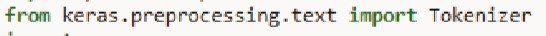
\includegraphics[width=0.5\textwidth]{figures/chapter7/no1.jpg}}
	\caption{Tokenizer}
	\label{no1}
	\end{figure}

\item Menjelaskan konsep dasar K-Fold Cross Validation
	\lstinputlisting[firstline=8, lastline=20]{src/chapter7/A2.py}
	\par Penjelasan kode listingg :
	\begin{enumerate}
	\item Membuat variabel kfold yang memanggil fungsi StratifiedKFold. StratifiedKFold itu sendiri ialah variasi Kfold yang mengembalikan lipatan bertingkat. Yang dimana pada kode program tersebut jumlah lipatannya adalah 5 atau dibagi menjadi 5 bagian.
	\item Membuat variabel split yang mempresentasikan variabel kfold untuk dibagi berdasarkan class.
	\end{enumerate}
	
	\par Berikut adalah gambar  \ref{no2} ilustrasi dari kosep dasar kfold.
		\begin{figure}[!hbtp]
		\centering
		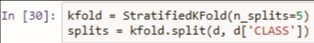
\includegraphics[scale=0.4]{figures/chapter7/no2.jpg}
		\caption{StratifiedKFold}
		\label{no2}
		\end{figure}

\item Jelaskan apa maksudnya kode program for train, test in splits, dilengkapi dengan ilustrasi atau gambar
	\par Maksudnya yaitu untuk menguji apakah setiap data pada dataset sudah di split dan tidak terjadi penumpukan. Yang dimana maksudnya di setiap class tidak akan muncul id yang sama. Ilustrasinya misalkan kita memiliki 5 jam tangan dengan model yang berbeda. Kemudian kita bagikan jam tersebut kepada teman, tentunya teman tersebut yang menerima jam tangan itu tidak memiliki jam yang sama modelnya.
 

\item Menjelaskan maksud kode program
	\lstinputlisting[firstline=8, lastline=20]{src/chapter7/A4.py}
	\par Dari kode program tersebut dapat dijelaskan bahwa membuat fungsi train dan test dengan menggunakan dataset yang hanya diambil kolom 'CONTENT' saja. iloc berfingsi sebagai pengindeksan posisi menggunakan integer.
	
	\par Berikut ilustrasi dari kode program tersebut, perhatikan gambar \ref{no4}.
		\begin{figure}[!hbtp]
		\centering
		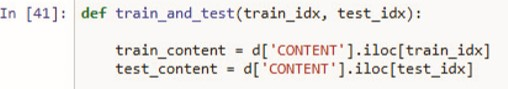
\includegraphics[scale=0.4]{figures/chapter7/no4.jpg}
		\caption{Ilustrasi Kode Program No.4}
		\label{no4}
		\end{figure}

\item Apa Maksud Dari Fungsi Tokenizer = Tokenizer(num words=2000) Dan Tokenizer.fit on texts(train content), Dilengkapi Dengan Ilustrasi Gambar
	\lstinputlisting[firstline=8, lastline=20]{src/chapter7/A5.py}
		
	\par Dari kode program  membuat variabel tokenizer untuk memanggil fungsi tokenizer agar dapat dilakukan vektorisasi dari kata. Dimana pada kode program pada baris pertama menggunakan 2000 kata atau 2000 kolom.
	
	
	\par Berikut adalah gambar  \ref{no5}  ilustrasi dari fungsi pada kode program tersebut.
	
		\begin{figure}[!hbtp]
		\centering
		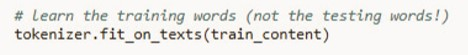
\includegraphics[scale=0.4]{figures/chapter7/no5.jpg}
		\caption{fungsi tokenizer}
		\label{no5}
		\end{figure}

\item  Apa Maksud Dari Fungsi d train inputs = tokenizer.texts to matrix(train content, mode=’tfidf ’) dan d test inputs = tokenizer.texts to matrix(test content, mode=’tfidf ’), Dilengkapi Dengan Ilustrasi Kode Dan Atau Gambar

	\lstinputlisting[firstline=8, lastline=20]{src/chapter7/A6.py}
		
	\par Dari fungsi pada kode program tersebut dapat dijelaskan bahwa :
	\begin{enumerate}
	\item Baris pertama membuat variabel d\_train\_inputs untuk memanggil fungsi tokrnizer dan merubah data train yang berupa teks ke dalam bentuk matrix dengan menggunakan model tfidf.
	\item Baris kedua membuat variabel d\_test\_inputs untuk memanggil fungsi tokrnizer dan merubah data test yang berupa teks ke dalam bentuk matrix dengan menggunakan model tfidf.
	\end{enumerate}
	
	\par Berikut adalah gambar \ref{no6} ilustrasi dari fungsi pada kode program tersebut.
	
		\begin{figure}[!hbtp]
		\centering
		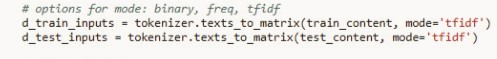
\includegraphics[scale=0.4]{figures/chapter7/no6.jpg}
		\caption{fungsi dtrain inputs}
		\label{no6}
		\end{figure}

\item Apa Maksud Dari Fungsi d train inputs = d train inputs/np.amax(np.absolute(d\_train) :
	\lstinputlisting[firstline=8, lastline=20]{src/chapter7/A7.py}
		
	\par Dari fungsi pada kode program tersebut dapat dijelaskan bahwa fungsi tersebut akan membagi matrix tfidf tadi dengan amax yaitu mengembalikan maksimum array atau maksimum sepanjang sumbu. Yang hasilnya akan dimasukan kedalam variabel d\_train\_inputs untuk data train dan d\_test\_inputs untuk data test dengan nominal absolut atau tanpa ada bilangan negatif dan koma.
	
	\par Berikut adalah gambar \ref{no7} ilustrasi dari fungsi pada kode program tersebut.
	
		\begin{figure}[!hbtp]
		\centering
		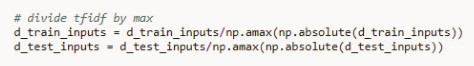
\includegraphics[scale=0.4]{figures/chapter7/no7.jpg}
		\caption{dtrain iinputs}
		\label{no7}
		\end{figure}

\item Jelaskan apa maksud dari fungsi d\_train\_outputs dan d\_test\_outputs, dilengkapi dengan ilustrasi atau gambar.
\lstinputlisting[firstline=8, lastline=20]{src/chapter7/A8.py}
		
	\par Dari fungsi pada kode program tersebut dapat dijelaskan bahwa fungsi tersebut ditujukan untuk melakukan one-hot encoding supaya bisa masuk dan digunakan pada neural network. One-hot encoding diambil dari 'CLASS' yang berarti hanya terdapat 2 neuron, yaitu satu nol(1,0) atau nol satu(0,1) karena pilihannya hanya ada dua (spam atau bukan).
	\par Berikut adalah gambar \ref{no8} ilustrasi dari fungsi pada kode program tersebut.
		\begin{figure}[!hbtp]
		\centering
		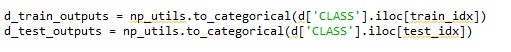
\includegraphics[scale=0.4]{figures/chapter7/no8.jpg}
		\caption{fungsi dtrain outputs}
		\label{no8}
		\end{figure}

\item Jelaskan apa maksud dari fungsi di listing 7.2 , Gambarkan ilustrasi Neural Networknya.
\lstinputlisting[firstline=8, lastline=20]{src/chapter7/A9.py}
	\par Dari fungsi pada kode program tersebut ditujukan untuk melakukan pemodelan dengan sequential, membandingkan setiap satu larik elemen dengan cara satu persatu secara beruntun. Dimana terdapat 512 neuron inputan dengan input shape 2000 vektor yang sudah dinormalisasi. Lalu model dilakukan aktivasi dengan fungsi 'relu'. Kemudian dilakukan pemotongan bobot supaya tidak overfitting sebesar 50 persen dari neuron inputan 512. Lalu pada layer output terdapat 2 neuron outputan yaitu nol(1,0) atau nol satu(0,1). Kemudian outputan tersebut diaktivasi menggunakan fungsi softmax (mencari nilai maximal).
	\par Berikut adalah gambar \ref{no9} ilustrasi dari fungsi pada kode program tersebut.
		\begin{figure}[!hbtp]
		\centering
		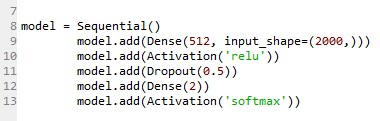
\includegraphics[scale=0.4]{figures/chapter7/no9.jpg}
		\caption{fungsi di listing 7.2}
		\label{no9}
		\end{figure}

\item Jelaskan apa maksud dari fungsi di listing 7.3 .
\lstinputlisting[firstline=8, lastline=20]{src/chapter7/A10.py}
	\par Dari fungsi pada kode program tersebut model yang telah dibuat selanjutnya dicompile dengan menggunakan algoritma optimisasi, fungsi loss, dan fungsi metrik.
	\par Berikut adalah gambar \ref{no10} ilustrasi dari fungsi pada kode program tersebut.
		\begin{figure}[!hbtp]
		\centering
		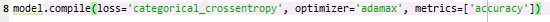
\includegraphics[scale=0.4]{figures/chapter7/no10.jpg}
		\caption{fungsi di listing 7.3}
		\label{no10}
		\end{figure}

\item Jelaskan apa itu Deep Learning.
	\par Deep Learning merupakan cabang dari Machine Learning atau bagian keluarga yang lebih luas dari method machine learning berdasarkan pada representasi data pembelajaran. Deep Learning menggunakan Deep Neural Network dalam menyelesaikan suatu masalah yang terjadi pada Machine Learning.

\item Jelaskan apa itu Deep Neural Network, dan apa bedanya dengan Deep Learning.
	\par Deep Neural Network atau DNN merupakan algoritma yang berbasis neural network yang digunakan untuk mengambil keputusan. Yang membedakan Deep Learning dengan  Deep Neural Network (DNN) adalah DNN merupakan algoritma yang digunakan pada Deep Learning, sedangkan Deep Learning merupakan model yang menggunakan algoritma DNN.

\item Jelaskan dengan ilustrasi gambar langkah per langkah bagaimana perhitungan algoritma konvolusi dengan ukuran stide (NPM mod 3 + 1) x (NPM mod 3 + 1) yang terdapat max pooling !

	\begin{itemize}
		\item Pertama tentukan nilai (x,y) dan (x1,y1)
		\item Nilai tersebut dibuat kedalam bentuk matrix
		\item Jika sudah berbentuk matrix lakukan perkalian antar baris dan deret
		\item Hasil perkalian tersebut dijumlahkan sehingga akan menghasilkan nilai matrix (3x3)
	\end{itemize}

	\subitem Untuk ilustrasi dapat dilihat pada figure \ref{no13}

	\begin{figure}[!htbp!]
		\centerline{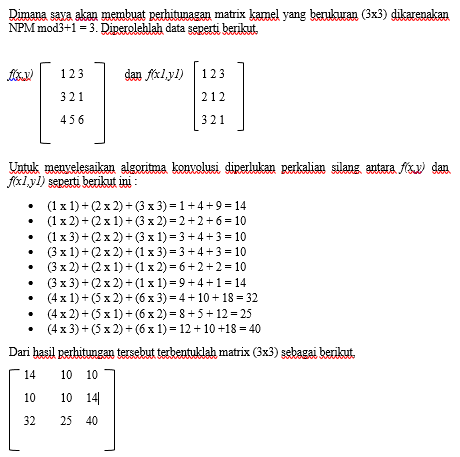
\includegraphics[width=0.5\textwidth]{figures/Chapter7/no13.png}}
		\caption{Algoritma Konvolusi Dengan Matrix (3x3).}
		\label{no13}
	\end{figure}	

\end{enumerate}





\subsection{Praktek}
\begin{enumerate}
\item Jelaskan kode program pada blok \# In[1]
	\par Berikut adalah kode program yang digunakan :
	\lstinputlisting[firstline=1, lastline=19, caption=Kode Program 1, label={71}]{src/chapter7/andri1.py}
	\par Dari kode listing pada kode program 1, dapat dijelaskan seperti berikut :
	\begin{itemize}
	\item Baris 1	: Melakukan pengimportan file csv
	\item Baris 2	: Melakukan pemanggilan atau memasukkan module image sebagai pil\_image dari library PIL
	\item Baris 3	: Melakukan pengimportan fungsi keras.processing.image 
	\end{itemize}
	\par Jalankan kode program tersebut, maka menghasilkan seperti pada gambar \ref{andri1}.
		\begin{figure}[!hbtp]
		\centering
		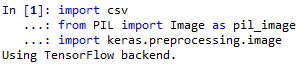
\includegraphics[scale=0.5]{figures/chapter7/andri1.jpg}
		\caption{Hasil kode program pada blok 1}
		\label{andri1}
		\end{figure}
	
\item Jelaskan kode program pada blok \# In[2]
	\par Berikut adalah kode program yang digunakan :
	\lstinputlisting[firstline=1, lastline=19, caption=Kode Program 2, label={72}]{src/chapter7/andri2.py}
	\par Dari kode listing pada kode program 2, dapat dijelaskan seperti berikut :
	\begin{itemize}
	\item Baris 1	: Membuat variabel imgs tanpa ada parameter di dalamnya
	\item Baris 2	: Membuat variabel classes tanpa ada parameter didalamnya
	\item Baris 3	: Membuka file csv dari HASYv2/hasy-data-labels.csv sebagai csvfile
	\item Baris 4	: Membuat variabel csvreader yang difungsikan untuk membaca dari file csv yang dimasukkan
	\item Baris 5	: Membuat variabel i dengan parameter 0 atau nilai 0
	\item Baris 6	: Digunakan untuk melakukan eksekusi baris dari pembacaan csv 
	\item Baris 7	: Mengaplikasikan atau menggunakan perintah "if" dengan variabel i lebih besar dari 0, yang selanjutnya akan dilanjutkan ke perintah berikutnya
	\item Baris 8	: Membuat variabel img yang berfungsi untuk mengubah image atau gambar menjadi bentuk array (bilangan) dari file HASYv2 yang dibuka dengan row berparameter 0.
	\item Baris 9	: Membuat variabel img dengan nilai bukan sama dengan 255.0
	\item Baris 10	: Mendefinisikan fungsi imgs.append yang digunakan untuk melakukan proses penggabungan data dengan file lain atau dataset lain yang telah ditentukan dengan 3 parameter yaitu row[0], row[2] dan variabel img.
	\item Baris 11	: Mendefinisikan fungsi append dari variabel classes dengan menggunakan parameter row[2].
	\item Baris 12	: Mengartikan i=i+1 yang dimana nilai sari variabel i akan ditambah 1 sehingga akan bernilai 1.
	\end{itemize}
	\par Jalankan kode program tersebut, maka menghasilkan seperti pada gambar \ref{andri2}.
		\begin{figure}[!hbtp]
		\centering
		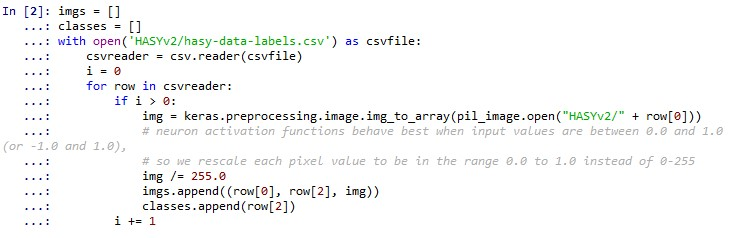
\includegraphics[scale=0.5]{figures/chapter7/andri2.jpg}
		\caption{Hasil kode program pada blok 2}
		\label{andri2}
		\end{figure}
	
\item Jelaskan kode program pada blok \# In[3]
	\par Berikut adalah kode program yang digunakan :
	\lstinputlisting[firstline=1, lastline=19, caption=Kode Program 3, label={73}]{src/chapter7/andri3.py}
	\par Dari kode listing pada kode program 3, dapat dijelaskan seperti berikut :
	\begin{itemize}
	\item Baris 1	: Memanggil dan menggunakan module random
	\item Baris 2	: Melakukan pengocokan menggunakan module random pada parameter variabel imgs
	\item Baris 3	: Membagi index data kedalam bentuk integer dengan mengalikan 0,8 dan len yang berfungsi mengembalikan jumlah item dalam datanya dari variabel imgs
	\item Baris 4	: Membuat variabel train yang digunakan untuk mengeksekusi imgs serta pemecahan index awal pada data untuk digunakan sebagai data training
	\item Baris 5	: Membuat variabel test yang digunakan untuk mengeksekusi imgs serta pemecahan index akhir pada data untuk digunakan sebagai data testing
	\end{itemize}
	\par Jalankan kode program tersebut, maka menghasilkan seperti pada gambar \ref{andri3}.
		\begin{figure}[!hbtp]
		\centering
		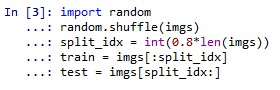
\includegraphics[scale=0.5]{figures/chapter7/andri3.jpg}
		\caption{Hasil kode program pada blok 3}
		\label{andri3}
		\end{figure}
	
\item Jelaskan kode program pada blok \# In[4]
	\par Berikut adalah kode program yang digunakan :
	\lstinputlisting[firstline=1, lastline=19, caption=Kode Program 4, label={74}]{src/chapter7/andri4.py}
	\par Dari kode listing pada kode program 4, dapat dijelaskan seperti berikut :
	\begin{itemize}
	\item Baris 1	: Melakukan import library numpy sebagai np
	\item Baris 2	: Membuat variabel train\_input untuk mengubah inputan menjadi array menggunakan fungsi np.asarray dan  fungsi list untuk mengkoleksi data yang dipilih serta data dapat diubah. Dan didalamnya melakukan penerapan fungsi map yang berfungsi untuk mengembalikan iterator dari data yang digunakan dan fungsi lamda pada row berparameter [2] difungsikan untuk membuat objek menjadi lebih kecil sehingga mudah dieksekusi dari variabel train.
	\item Baris 3	: Membuat variabel test\_input untuk mengubah inputan menjadi array menggunakan fungsi np.asarray dan  fungsi list untuk mengkoleksi data yang dipilih serta data dapat diubah. Dan didalamnya melakukan penerapan fungsi map yang berfungsi untuk mengembalikan iterator dari data yang digunakan dan fungsi lamda pada row berparameter [2] difungsikan untuk membuat objek menjadi lebih kecil sehingga mudah dieksekusi dari variabel test.
	\item Baris 4	: Membuat variabel train\_input untuk mengubah inputan menjadi array menggunakan fungsi np.asarray dan  fungsi list untuk mengkoleksi data yang dipilih serta data dapat diubah. Dan didalamnya melakukan penerapan fungsi map yang berfungsi untuk mengembalikan iterator dari data yang digunakan dan fungsi lamda pada row berparameter [1] difungsikan untuk membuat objek menjadi lebih kecil sehingga mudah dieksekusi dari variabel train.
	\item Baris 5	: Membuat variabel test\_input untuk mengubah inputan menjadi array menggunakan fungsi np.asarray dan  fungsi list untuk mengkoleksi data yang dipilih serta data dapat diubah. Dan didalamnya melakukan penerapan fungsi map yang berfungsi untuk mengembalikan iterator dari data yang digunakan dan fungsi lamda pada row berparameter [1] difungsikan untuk membuat objek menjadi lebih kecil sehingga mudah dieksekusi dari variabel test.
	\end{itemize}
	\par Jalankan kode program tersebut, maka menghasilkan seperti pada gambar \ref{andri4}.
		\begin{figure}[!hbtp]
		\centering
		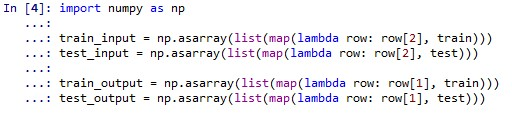
\includegraphics[scale=0.5]{figures/chapter7/andri4.jpg}
		\caption{Hasil kode program pada blok 4}
		\label{andri4}
		\end{figure}
	
\item Jelaskan kode program pada blok \# In[5]
	\par Berikut adalah kode program yang digunakan :
	\lstinputlisting[firstline=1, lastline=19, caption=Kode Program 5, label={75}]{src/chapter7/andri5.py}
	\par Dari kode listing pada kode program 5, dapat dijelaskan seperti berikut :
	\begin{itemize}
	\item Baris 1	: Menggunakan fungsi LabelEncoder dari sklearn.processing yang berfungsi untuk menormalkan label dimana label encoder hanya didefinisikan dengan nilai antara 0 dan -1.
	\item Baris 2	: Menggunakan fungsi OneHotEncoder dari sklearn.processing yang berfungsi untuk mendefinisikan fitur input yang dimana mengambil nilai dalam kisaran [0, nilai maksimal].
	\end{itemize}
	\par Jalankan kode program tersebut, maka menghasilkan seperti pada gambar \ref{andri5}.
		\begin{figure}[!hbtp]
		\centering
		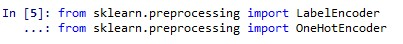
\includegraphics[scale=0.5]{figures/chapter7/andri5.jpg}
		\caption{Hasil kode program pada blok 5}
		\label{andri5}
		\end{figure}
	
\item Jelaskan kode program pada blok \# In[6]
	\par Berikut adalah kode program yang digunakan :
	\lstinputlisting[firstline=1, lastline=19, caption=Kode Program 6, label={75}]{src/chapter7/andri6.py}
	\par Dari kode listing pada kode program 6, dapat dijelaskan seperti berikut :
	\begin{itemize}
	\item Baris 1	: Membuat variabel label\_encoder dengan penerapan modul / fungsi LabelEncoder tanpa parameter
	\item Baris 2	: Membuat variabel integer\_encoded dengan penerapan fungsi label\_encoder.fit\_transform yang berfungsi untuk melakukan ekstrasi fitur object dari variabel classes yang akan mengembalikan beberapa data yang diubah kembali.
	\end{itemize}
	\par Jalankan kode program tersebut, maka menghasilkan seperti pada gambar \ref{andri6}.
		\begin{figure}[!hbtp]
		\centering
		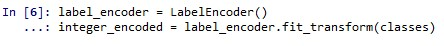
\includegraphics[scale=0.5]{figures/chapter7/andri6.jpg}
		\caption{Hasil kode program pada blok 6}
		\label{andri6}
		\end{figure}

\item Jelaskan kode program pada blok \# In[7]
	\par Berikut adalah kode program yang digunakan :
	\lstinputlisting[firstline=1, lastline=19, caption=Kode Program 7, label={77}]{src/chapter7/andri7.py}
	\par Dari kode listing pada kode program 7, dapat dijelaskan seperti berikut :
	\begin{itemize}
	\item Baris 1	: Membuat variabel onehot\_encoder yang memanggil fungsi OneHotEncoder tanpa mengembalikan matriks karena sparse=false.
	\item Baris 2	: Membuat variabel integer\_encoded memanggil variabel integer\_encoded pada kode program 6 untuk dieksekusi memberikan bentuk baru ke array tanpa mengubah datanya dari mengembalikan panjang nilai dari integer\_encoded.
	\item Baris 3	: Onehotencoding melakukan fitting pada integer\_encoded.
	\end{itemize}
	\par Jalankan kode program tersebut, maka menghasilkan seperti pada gambar \ref{andri7}.
		\begin{figure}[!hbtp]
		\centering
		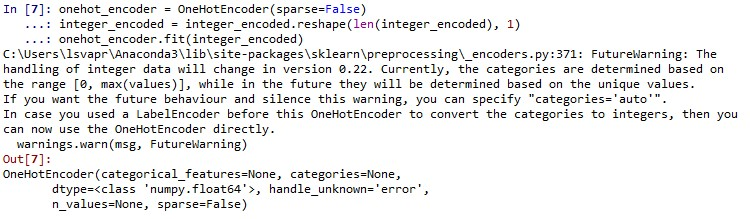
\includegraphics[scale=0.5]{figures/chapter7/andri7.jpg}
		\caption{Hasil kode program pada blok 7}
		\label{andri7}
		\end{figure}

\item Jelaskan kode program pada blok \# In[8]
	\par Berikut adalah kode program yang digunakan :
	\lstinputlisting[firstline=1, lastline=19, caption=Kode Program 8, label={78}]{src/chapter7/andri8.py}
	\par Dari kode listing pada kode program 8, dapat dijelaskan seperti berikut :
	\begin{itemize}
	\item Baris 1	: Membuat variabel train\_output\_int yang mengeksekusi label\_encoder dengan mengubah nilai dari parameter variabel train\_output.
	\item Baris 2	: Membuat variabel train\_output yang mengeksekusi variabel onehot\_encoder dari kode program 7 dengan mengubah nilai dari variabel parameter train\_output\_int yang datanya sudah diubah kedalam bentuk array dan panjang nilai dari train\_output\_int telah dikembalikan.
	\item Baris 3	: Membuat variabel test\_output\_int yang mengeksekusi label\_encoder dengan mengubah nilai dari parameter variabel test\_output.
	\item Baris 4	: Membuat variabel test\_output yang mengeksekusi variabel onehot\_encoder dari kode program 7 dengan mengubah nilai dari variabel parameter test\_output\_int yang datanya sudah diubah kedalam bentuk array dan panjang nilai dari test\_output\_int telah dikembalikan.
	\item Baris 5	: Membuat variabel num\_classes untuk mengetahui jumlah class dari lebel\_encoder
	\item Baris 6	: Perintah print digunakan untuk memunculkan hasil dari variabel num\_classes
	\end{itemize}
	\par Jalankan kode program tersebut, maka menghasilkan seperti pada gambar \ref{andri8}.
		\begin{figure}[!hbtp]
		\centering
		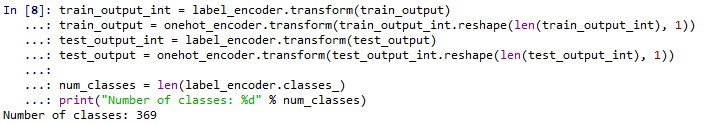
\includegraphics[scale=0.5]{figures/chapter7/andri8.jpg}
		\caption{Hasil kode program pada blok 8}
		\label{andri8}
		\end{figure}
		
\item Jelaskan kode program pada blok \# In[9]
	\par Berikut adalah kode program yang digunakan :
	\lstinputlisting[firstline=1, lastline=19, caption=Kode Program 9, label={79}]{src/chapter7/andri9.py}
	\par Dari kode listing pada kode program 9, dapat dijelaskan seperti berikut :
	\begin{itemize}
	\item Baris 1	: Memanggil atau melakukan importing fungsi model sequential dari library keras.
	\item Baris 2	: Memanggil atau melakukan importing fungsi layer dense, dropout, dan flatten dari library keras.
	\item Baris 3	: Memanggil atau melakukan importing fungsi layer Conv2D dan MaxPooling2D dari library keras.
	\end{itemize}
	\par Jalankan kode program tersebut, maka menghasilkan seperti pada gambar \ref{andri9}.
		\begin{figure}[!hbtp]
		\centering
		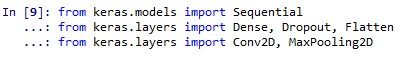
\includegraphics[scale=0.5]{figures/chapter7/andri9.jpg}
		\caption{Hasil kode program pada blok 9}
		\label{andri9}
		\end{figure}

\item Jelaskan kode program pada blok \# In[10]
\par Berikut adalah kode program yang digunakan :
	\lstinputlisting[firstline=1, lastline=19, caption=Kode Program 10, label={710}]{src/chapter7/andri10.py}
	\par Dari kode listing pada kode program 10, dapat dijelaskan seperti berikut :
	\begin{itemize}
	\item Baris 1	: Melakukan pemodelan Sequential.
	\item Baris 2	: Menambahkan Konvolusi 2D dengan 32 filter konvolusi menggunakan matriks kernel berukuran 3x3 dengan algoritma activation adalah relu, dimana data diambil dari train\_input yang dimulai dari baris ke-nol.
	\item Baris 3	: Menambahkan Max Pooling dengan matriks 2x2.
	\item Baris 4	: Melakukan penambahkan konvolusi 2D lagi dengan 32 filter konvolusi menggunakan matrik kernel masing-masing berukuran 3x3 dengan algoritam activation relu.
	\item Baris 5	: Melakukan penambahan lagi Max Pooling dengan matriks 2x2.
	\item Baris 6	: Melakukan perataan pada inputan model.
	\item Baris 7	: Mendefinisikan inputan dengan 1024 neuron dan melakukan aktivasi menggunakan algoritma tanh.
	\item Baris 8	: Dropout dilakukan untuk melakukan pemotongan pada cabang yang terdiri dari pengaturan secara acak tingkat pecahan unit input ke 0 pada setiap pembaruan selama waktu pelatihan, yang membantu mencegah overfitting sebesar 50\%.
	\item Baris 9	: Pada output layer menggunakan data dari variabel num\_classes dan menggunakan fungsi aktivasi softmax.
	\item Baris 10 	: Melkukan konfigurasi proses pembelajaran, yang dilakukan melalui metode compile, sebelum melatih suatu model.
	\item Baris 11	: Menampilkan hasil representasi ringkasan dari model yang telah dibuat.
	\end{itemize}
	\par Jalankan kode program tersebut, maka menghasilkan seperti pada gambar \ref{andri10}.
		\begin{figure}[!hbtp]
		\centering
		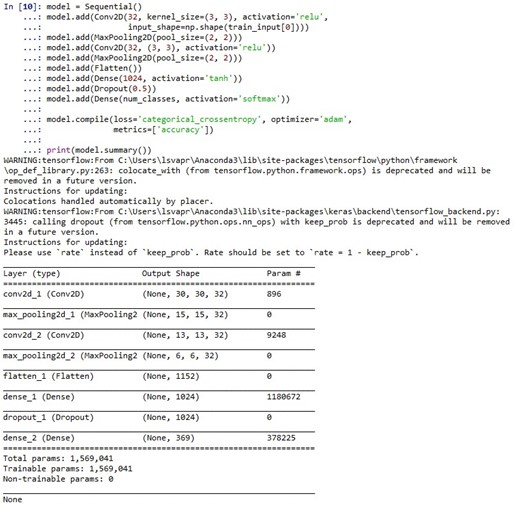
\includegraphics[scale=0.5]{figures/chapter7/andri10.jpg}
		\caption{Hasil kode program pada blok 10}
		\label{7B10}
		\end{figure}

\item Jelaskan kode program pada blok \# In[11]
	\par Berikut adalah kode program yang digunakan :
	\lstinputlisting[firstline=1, lastline=19, caption=Kode Program 11, label={711}]{src/chapter7/andri11.py}
	\par Dari kode listing pada kode program 11, dapat dijelaskan seperti berikut :
	\begin{itemize}
	\item Baris 1	: Melakukan importing library keras.callbacks yang memiliki fungsi penulisan log untuk TensorBoard, yang memungkinkan untuk memvisualisasikan grafik dinamis dari training dan metrik pengujian.
	\item Baris 2	: Membuat variabel tenserboard yang menggunakan fungsi TensorBoard dari keras.callbacks yang berfungsi sebagai alat visualisasi yang telah disediakan oleh TensorFlow. Kemudian untuk fungsi log\_dir memanggil data yaitu './logs/mnist-style' dari direktori.
	\end{itemize}
	\par Jalankan kode program tersebut, maka menghasilkan seperti pada gambar \ref{andri11}.
		\begin{figure}[!hbtp]
		\centering
		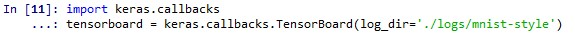
\includegraphics[scale=0.5]{figures/chapter7/andri11.jpg}
		\caption{Hasil kode program pada blok 11}
		\label{andri11}
		\end{figure}

\item Jelaskan kode program pada blok \# In[12]
	\par Berikut adalah kode program yang digunakan :
	\lstinputlisting[firstline=1, lastline=19, caption=Kode Program 12, label={712}]{src/chapter7/andri12.py}
	\par Dari kode listing pada kode program 12, dapat dijelaskan seperti berikut :
	\begin{itemize}
	\item Baris 1	: Menerapkan fungsi model.fit yang didalamnya memproses train\_input, train\_output dengan batch\_size, epochs, verbose, validation\_split, dan callbacks.
		\begin{itemize}
		\item Batch\_size merupakan jumlah sampel per pembaharuan sampel dari data yang diolah, sehingga apabila batch\_sizenya tidak ditemukan maka otomatis akan dijadikan nilai 32.
		\item Epochs berfungsi untuk melakukan perulangan dimana perulangan dari berapa kali nilai yang digunakan untuk data, dan jumlahnya ialah 10.
		\item Verbose digunakan sebagai opsi untuk menghasilkan informasi logging dari data yang ditentukan dengan nilai 2.
		\item Validation\_split berfungsi untuk memecah nilai dari perhitungan dengan validasinya sebesar 0,2. (Fraksi data pelatihan untuk digunakan sebagai data validasi).
		\item Callsbacks mengeksekusi tensorboard yang berfungsi untuk memvisualisasikan parameter training, metrik, hiperparameter pada nilai/data yang diproses.
		\end{itemize}	
	\item Baris 2	: Membuat variabel score dengan menggunakan fungsi evaluate dari model yang ada dengan variabel parameter test\_input, tst\_output dan verbose=2 yang berfungsi memprediksi output untuk input yang diberikan dan kemudian menghitung fungsi metrik yang ditentukan dalam modelnya.
	\item Baris 3	: Mencetak variabel score optimasi dari test dengan ketentuan nilai parameter 0
	\item Baris 4	: Mencetak variabel score akurasi dari test dengan ketentuan nilai parameter 1
	\end{itemize}
	\par Jalankan kode program tersebut, maka menghasilkan seperti pada gambar \ref{andri12}.
		\begin{figure}[!hbtp]
		\centering
		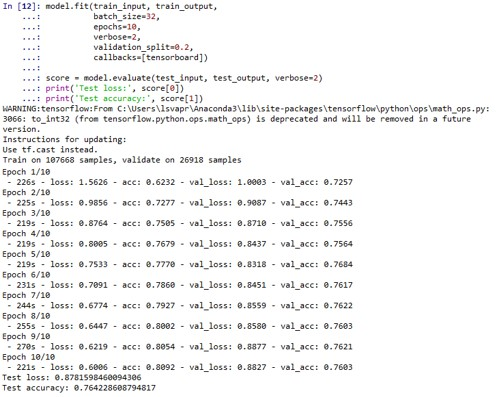
\includegraphics[scale=0.5]{figures/chapter7/andri12.jpg}
		\caption{Hasil kode program pada blok 12}
		\label{andri12}
		\end{figure}

\item Jelaskan kode program pada blok \# In[13]
	\par Berikut adalah kode program yang digunakan :
	\lstinputlisting[firstline=1, lastline=19, caption=Kode Program 13, label={713}]{src/chapter7/andri13.py}
	\par Dari kode listing pada kode program 13, dapat dijelaskan seperti berikut :
	\begin{itemize}
	\item Baris 1	: Melakukan importing modul time.
	\item Baris 2	: Membuat variabel result berisikan array kosong.
	\item Baris 3	: Menggunakan convolution 2D yang dimana akan memiliki 1 atau 2 layer
	\item Baris 4	: Mendefinisikan dense\_size dengan ukuran 128, 256, 512, 1024, 2048
	\item Baris 5	: Mendefinsikan drop\_out dengan 0, 25\%, 50\%, dan 75\%
	\item Baris 6	: Melakukan pemodelan Sequential
	\item Baris 7	: Untuk i dalam cakupan conv2d\_count
	\item Baris 8	: Jika ini adalah layer pertama, kita perlu memasukkan bentuk input.
	\item Baris 9	: Kalau tidak kita hanya akan menambahkan layer.
	\item Baris 10	: Kemudian, setelah menambahkan layer konvolusi, akan dilakukan hal yang sama dengan max pooling.
	\item Baris 11	: Lalu, melakukan perataan atau flatten dan menambahkan dense size ukuran apa pun yang berasal dari dense\_size. Dimana akan selalu menggunakan algoritma tanh.
	\item Baris 12	: Jika dropout digunakan, maka akan menambahkan layer dropout. Katakanlah 50\% dilakukan dropout, bahwa setiap kali ia memperbarui bobot setelah setiap batch, ada peluang 50\% untuk setiap bobot yang tidak akan diperbarui dan menempatkannya di antara dua lapisan padat untuk diaktivasi serta melindunginya dari overfitting.
	\item Baris 13	:  Lapisan terakhir akan selalu menjadi jumlah kelas karena itu harus, dan menggunakan softmax. Dan dikompilasi dengan cara yang sama.
	\item Baris 14	:  Mengatur direktori log yang berbeda untuk TensorBoard sehingga dapat membedakan konfigurasi yang berbeda.
	\item Baris 15	: Variabel start akan memanggil modul time atau waktu
	\item Baris 16	: Melakukan fit atau compile 
	\item Baris 17	: Melakukan scoring dengan .evaluate yang berfungsi menampilkan data loss dan accuracy dari model
	\item Baris 18	: end merupakan variabel untuk melihat waktu akhir pada saat pemodelan berhasil dilakukan.
	\item Baris 19	: Menampilkan hasil dari run skrip
	\end{itemize}
	\par Jalankan kode program tersebut, maka menghasilkan seperti pada gambar \ref{andri13}.
		\begin{figure}[!hbtp]
		\centering
		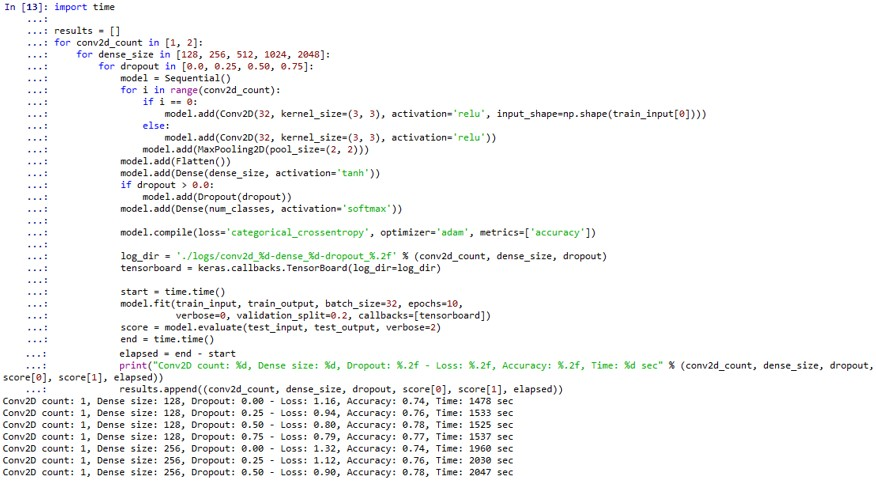
\includegraphics[scale=0.5]{figures/chapter7/andri13.jpg}
		\caption{Hasil kode program pada blok 13}
		\label{andri13}
		\end{figure}

\item Jelaskan kode program pada blok \# In[14]
	\par Berikut adalah kode program yang digunakan :
	\lstinputlisting[firstline=1, lastline=19, caption=Kode Program 14, label={714}]{src/chapter7/andri14.py}
	\par Dari kode listing pada kode program 14, dapat dijelaskan seperti berikut :
	\begin{itemize}
	\item Baris 1: Membuat model dengan menggunakan pemodelan Sequential
	\item Baris 2: Pada layer pertama melakukan penambahan Convolutio 2D dengan dimensi 32, dan ukuran matriks kernel 3x3 dengan menggunkan fungsi aktivasi relu dan menampilkan input\_shape
	\item Baris 3: Melakukan Max Pooling 2D dengan ukuran matriks 2x2
	\item Baris 4: Pada layer kedua, dilakukan convolusi lagi dengan kriteria yang sama tanpa ada penambahan input, hal ini dilakukan untuk mendapatkan data terbaik
	\item Baris 5: Melakukan Flatten untuk meratakan inputan
	\item Baris 6: Menambahkan dense input sebanyak 128 neuron dengan menggunakan fungsi aktivasi tanh.
	\item Baris 7: Melakukan Dropout sebanyak 50\% untuk menghindari overfitting
	\item Baris 8: Menambahkan dense pada model untuk output dimana layer ini akan menjadi jumlah dari class yang ada.
	\item Baris 9: Melakukan compiling dari model yang telah didefinisikan 
	\item Baris 10: Menampilkan ringkasan dari pemodelan yang dilakukan 
	\end{itemize}
	\par Jalankan kode program tersebut, maka menghasilkan seperti pada gambar \ref{andri14}.
		\begin{figure}[!hbtp]
		\centering
		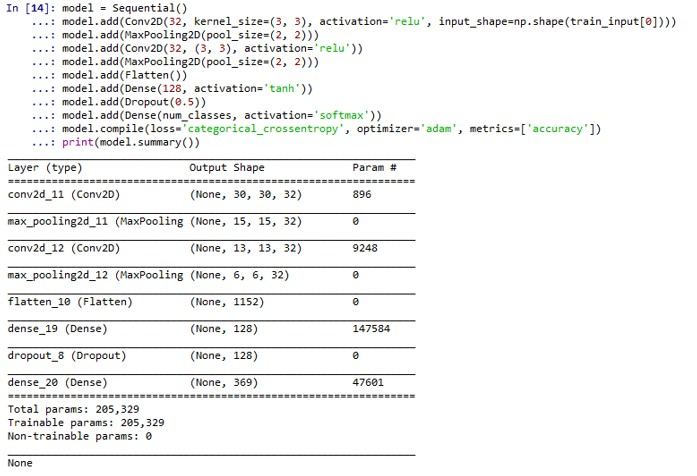
\includegraphics[scale=0.5]{figures/chapter7/andri14.jpg}
		\caption{Hasil kode program pada blok 14}
		\label{andri14}
		\end{figure}

\item Jelaskan kode program pada blok \# In[15]
\par Berikut adalah kode program yang digunakan :
	\lstinputlisting[firstline=1, lastline=19, caption=Kode Program 15, label={715}]{src/chapter7/andri15.py}
	\par Dari kode listing pada kode program 15, dapat dijelaskan seperti berikut :
	\begin{itemize}
	\item Baris 1: Melakukan fit atau fitting (pencocokan data) dengan penggabungan dari data train dan test agar dapat dilakukan pelatihan untuk jaringan pada smeua data yang dimiliki.
	\end{itemize}
	\par Jalankan kode program tersebut, maka menghasilkan seperti pada gambar \ref{andri15}.
		\begin{figure}[!hbtp]
		\centering
		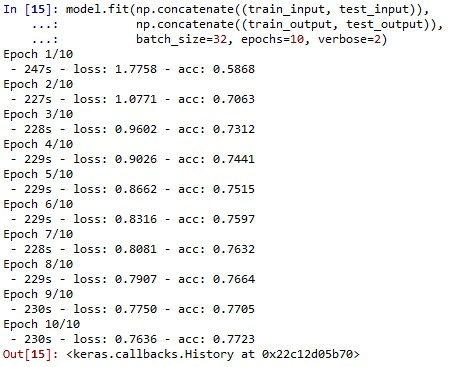
\includegraphics[scale=0.5]{figures/chapter7/andri15.jpg}
		\caption{Hasil kode program pada blok 15}
		\label{andri15}
		\end{figure}

\item Jelaskan kode program pada blok \# In[16]
\par Berikut adalah kode program yang digunakan :
	\lstinputlisting[firstline=1, lastline=19, caption=Kode Program 16, label={716}]{src/chapter7/andri16.py}
	\par Dari kode listing pada kode program 16, dapat dijelaskan seperti berikut :
	\begin{itemize}
	\item Baris 1	: Menyimpan model sebagai mathsymbols.model
	\end{itemize}
	\par Jalankan kode program tersebut, maka menghasilkan seperti pada gambar \ref{andri16}.
		\begin{figure}[!hbtp]
		\centering
		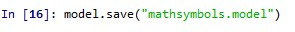
\includegraphics[scale=0.5]{figures/chapter7/andri16.jpg}
		\caption{Hasil kode program pada blok 16}
		\label{andri16}
		\end{figure}

\item Jelaskan kode program pada blok \# In[17]
	\par Berikut adalah kode program yang digunakan :
	\lstinputlisting[firstline=1, lastline=19, caption=Kode Program 17, label={717}]{src/chapter7/andri17.py}
	\par Dari kode listing pada kode program 17, dapat dijelaskan seperti berikut :
	\begin{itemize}
	\item Baris 1	: Menyimpan array dari label\_encoder.classes\_ ke file biner dalam format NumPy .npy.
	\end{itemize}
	\par Jalankan kode program tersebut, maka menghasilkan seperti pada gambar \ref{andri17}.
		\begin{figure}[!hbtp]
		\centering
		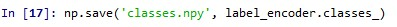
\includegraphics[scale=0.5]{figures/chapter7/andri17.jpg}
		\caption{Hasil kode program pada blok 17}
		\label{andri17}
		\end{figure}

\item Jelaskan kode program pada blok \# In[18]
	\par Berikut adalah kode program yang digunakan :
	\lstinputlisting[firstline=1, lastline=19, caption=Kode Program 18, label={718}]{src/chapter7/andri18.py}
	\par Dari kode listing pada kode program 18, dapat dijelaskan seperti berikut :
	\begin{itemize}
	\item Baris 1	: Melakukan importing modul models dari library keras
	\item Baris 2	: Membuat variabel model2 untuk memanggil dan membaca file mathsymbols.model
	\item Baris 3	: Berfungsi untuk menampilkan dan memeriksa hasil dari variabel parameter model2
	\end{itemize}
	\par Jalankan kode program tersebut, maka menghasilkan seperti pada gambar \ref{andri18}.
		\begin{figure}[!hbtp]
		\centering
		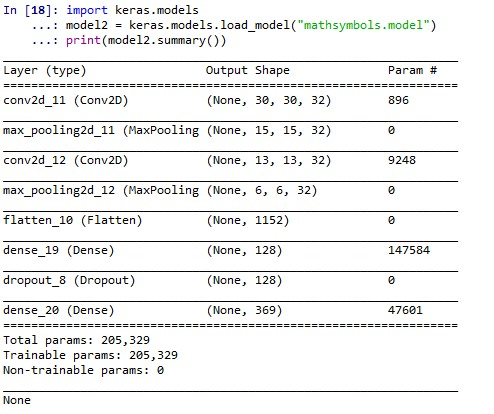
\includegraphics[scale=0.5]{figures/chapter7/andri18.jpg}
		\caption{Hasil kode program pada blok 18}
		\label{andri18}
		\end{figure}

\item Jelaskan kode program pada blok \# In[19]
	\par Berikut adalah kode program yang digunakan :
	\lstinputlisting[firstline=1, lastline=19, caption=Kode Program 19, label={719}]{src/chapter7/andri19.py}
	\par Dari kode listing pada kode program 19, dapat dijelaskan seperti berikut :
	\begin{itemize}
	\item Baris 1	: Membuat variabel label\_encoder2 yang melakukan pemanggilan fungsi LabelEncoder untuk melakukan penyandian pada label dengan nilai antara 1 dan 0
	\item Baris 2	: Variabel label\_encoder akan memanggil class yang telah disimpan sebelumnya.
	\item Baris 3	: Function Predict akan mengubah gambar kedalam bentuk array
	\item Baris 4	: Variabel prediction akan melakukan prediksi untuk model2 dengan Memberikan bentuk baru tanpa mengubah data dari variabel newimg dengan bentuk array 4D.
	\item Baris 5	: Variabel inverted akan mencari nilai tertinggi output dari hasil prediksi.
	\end{itemize}
	\par Jalankan kode program tersebut, maka menghasilkan seperti pada gambar \ref{andri19}.
		\begin{figure}[!hbtp]
		\centering
		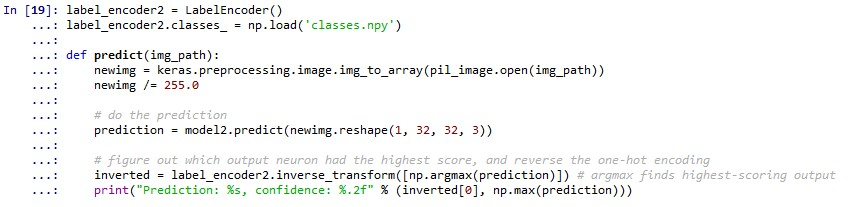
\includegraphics[scale=0.5]{figures/chapter7/andri19.jpg}
		\caption{Hasil kode program pada blok 19}
		\label{andri19}
		\end{figure}
		
\item Jelaskan kode program pada blok \# In[20]
	\par Berikut adalah kode program yang digunakan :
	\lstinputlisting[firstline=1, lastline=19, caption=Kode Program 20, label={720}]{src/chapter7/andri20.py}
	\par Dari kode listing pada kode program 20, dapat dijelaskan seperti berikut :
	\begin{itemize}
	\item Baris 1	: Melakukan prediksi terhadap file v2-00010.png yang diambil dari direktori
	\item Baris 2	: Melakukan prediksi terhadap file v2-00500.png yang diambil dari direktori
	\item Baris 3	: Melakukan prediksi terhadap file v2-00700.png yang diambil dari direktori
	\end{itemize}
	\par Jalankan kode program tersebut, maka menghasilkan seperti pada gambar \ref{andri20}.
		\begin{figure}[!hbtp]
		\centering
		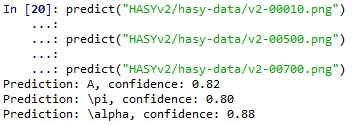
\includegraphics[scale=0.5]{figures/chapter7/andri20.jpg}
		\caption{Hasil kode program pada blok 20}
		\label{andri20}
		\end{figure}

\end{enumerate}


\subsection{Penanganan Error}
Dari praktek pemrograman yang dilakukan di modul ini, error yang kita dapatkan(hasil komputer sendiri) di dokumentasikan dan di selesaikan(nilai 5 per error yang ditangani. Untuk hari kedua):

\begin{enumerate}
\lstinputlisting[firstline=8, lastline=20]{src/chapter7/error.py}
	\item skrinsut error
		\begin{figure}[!htbp!]
		\centerline{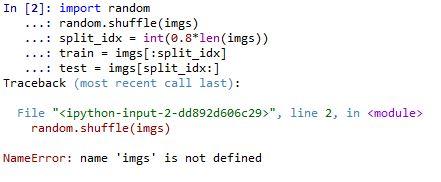
\includegraphics[width=0.5\textwidth]{figures/chapter7/error.jpg}}
		\caption{Screenshot Error}
		\label{Error}
	\end{figure}	
		
	\item Tuliskan kode error dan jenis errornya
		\begin{enumerate}
		\item Kode Error  :
			\begin{itemize}
				\item Kode error : "Name Error" name 'imgs'  is not defined"
				\item Jenis error : Jenis Error: Images tidak terdefinisi
			\end{itemize}
		\end{enumerate}

	\item Solusi pemecahan masalah error
	\par Menentukan atau memebuka file explorer dari file yang ditempatkan atau disesuaikan dengan letak filenya.
		
		
\end{enumerate}